\documentclass{beamer}

% Theme
\usetheme{Madrid}
\usecolortheme{default}

% Packages
\usepackage{amsmath,amssymb,amsfonts}
\usepackage{graphicx}
\usepackage{gvv}
\usepackage{xcolor}
\usepackage{tikz}
\usepackage{tkz-euclide}
\usepackage{array}
\usepackage{multirow}
\usepackage{longtable}
\usepackage{lscape}
\usepackage{listings}
\lstset{
    basicstyle=\ttfamily\small,
    keywordstyle=\color{blue},
    commentstyle=\color{gray},
    stringstyle=\color{red},
    showstringspaces=false,
    breaklines=true
}

\title{4.2.22}
\author{EE25BTECH11019 -- Darji Vivek M.}
\date{}

\begin{document}

\begin{frame}
\begin{titlepage}

\end{titlepage}
\end{frame}

\begin{frame}{Question}
\textbf{Question:}\\
Show that the two lines
\[
a_1 x + b_1 y + c_1 = 0,\qquad a_2 x + b_2 y + c_2 = 0
\]
where $b_1 b_2 \neq 0$ are parallel if 
\[
\frac{a_1}{b_1}=\frac{a_2}{b_2}.
\]
\end{frame}


\begin{frame}{Solution}

First form the matrix equation
\begin{align}
\myvec{a_1 & b_1\\ a_2 & b_2}\myvec{x\\y} 
= -\myvec{c_1\\c_2}.
\end{align}

Augmented matrix:
\begin{align}
\augvec{2}{1}{
a_1 & b_1 & -c_1\\
a_2 & b_2 & -c_2
}.
\end{align}

Perform row-reduction:
\begin{align}
R_2 \to R_2 - \frac{a_2}{a_1}R_1
\implies
\augvec{2}{1}{
a_1 & b_1 & -c_1\\
0 & \frac{a_1b_2 - a_2b_1}{a_1} & -c_2 + \frac{a_2c_1}{a_1}
}.
\end{align}
\end{frame}


\begin{frame}{Solution}
For two lines to be parallel, the coefficient matrix must have rank 1 and the augmented matrix must have rank 2
Thus,
\begin{align}
a_1b_2 - a_2b_1 = 0.
\end{align}

\(\therefore\) The two lines are parallel if
\begin{align}
\frac{a_1}{b_1} = \frac{a_2}{b_2}, \quad \text{where } b_1b_2 \neq 0.
\end{align}

\end{frame}


\begin{frame}{Pyhton plot}
\begin{figure}[h!]
    \centering
    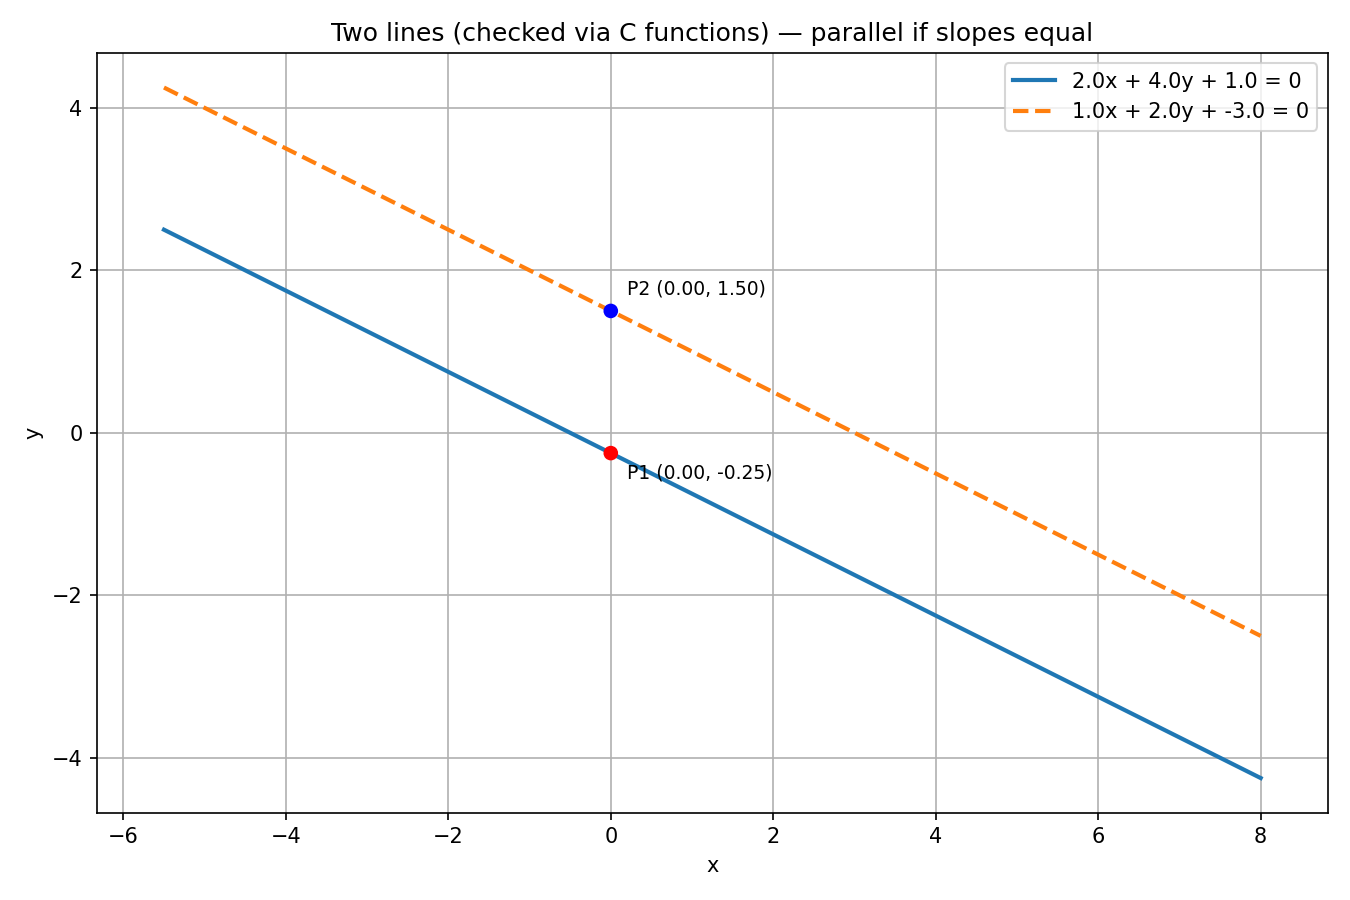
\includegraphics[width=0.75\textwidth]{figs/6.png}
    \caption{parallel lines}
    \label{fig:example_image}
    
\end{figure}
\end{frame}
% --- C Code Frame ---
\begin{frame}[fragile]{C Code: parallel\_funcs.c}
\begin{lstlisting}[language=C, basicstyle=\ttfamily\scriptsize, keywordstyle=\color{blue}]
#include <stdio.h>
#include <math.h>

#define EPS 1e-9

// Return 1 if lines are parallel, else 0
int is_parallel(double a1, double b1, double a2, double b2) {
    double det = a1*b2 - a2*b1;
    if (fabs(det) < EPS) return 1;
    return 0;
}

// Evaluate line a*x + b*y + c = 0
void eval_line(double a, double b, double c,
               double *x_in, double *y_out, int n) {
    for (int i = 0; i < n; ++i) {
        y_out[i] = (-a * x_in[i] - c) / b;
    }
}
\end{lstlisting}
\end{frame}

% --- Python ctypes Frame 1 ---
\begin{frame}[fragile]{Python: Load C Library}
\begin{lstlisting}[language=Python, basicstyle=\ttfamily\scriptsize, keywordstyle=\color{blue}]
import ctypes, numpy as np, matplotlib.pyplot as plt, os

libpath = os.path.join('.', 'libparallel.so')
lib = ctypes.CDLL(libpath)

# Signatures
lib.is_parallel.argtypes = [ctypes.c_double, ctypes.c_double,
                            ctypes.c_double, ctypes.c_double]
lib.is_parallel.restype = ctypes.c_int
lib.eval_line.argtypes = [ctypes.c_double, ctypes.c_double, ctypes.c_double,
                          ctypes.POINTER(ctypes.c_double),
                          ctypes.POINTER(ctypes.c_double),
                          ctypes.c_int]
lib.eval_line.restype = None
\end{lstlisting}
\end{frame}

% --- Python ctypes Frame 2 ---
\begin{frame}[fragile]{Python: Check Parallelism}
\begin{lstlisting}[language=Python, basicstyle=\ttfamily\scriptsize, keywordstyle=\color{blue}]
def check_parallel(a1, b1, a2, b2):
    return bool(lib.is_parallel(a1, b1, a2, b2))

def eval_line(a, b, c, xs):
    n = len(xs)
    XTYPE = ctypes.c_double * n
    x_arr = XTYPE(*xs)
    y_arr = XTYPE()
    lib.eval_line(a, b, c, x_arr, y_arr, n)
    return np.array([y_arr[i] for i in range(n)])

# Example lines
a1, b1, c1 = 2.0, 4.0, 1.0
a2, b2, c2 = 1.0, 2.0, -3.0
print("Are parallel? ->", check_parallel(a1, b1, a2, b2))
\end{lstlisting}
\end{frame}

% --- Python Plotting Frame ---
\begin{frame}[fragile]{Python: Plotting Lines}
\begin{lstlisting}[language=Python, basicstyle=\ttfamily\scriptsize, keywordstyle=\color{blue}]
xs = np.linspace(-10, 10, 600)
ys1 = eval_line(a1, b1, c1, xs)
ys2 = eval_line(a2, b2, c2, xs)

plt.figure()
plt.plot(xs, ys1, label=f'{a1}x+{b1}y+{c1}=0')
plt.plot(xs, ys2, '--', label=f'{a2}x+{b2}y+{c2}=0')
plt.legend(); plt.grid(True)
plt.axis('equal')
plt.savefig('parallel_lines_ctypes.png', dpi=150)
plt.show()
\end{lstlisting}
\end{frame}


\end{document}
